\addtocontents{toc}{\protect\vspace{\beforebibskip}} % Place slightly below the rest of the document content in the table


%************************************************
\chapter{Desenvolvimento}
\label{ch:desenvolvimento}
%************************************************


O corpo do relatório compõe, normalmente, a parte mais extensa do relatório, e contém todos os conteúdos necessários para que o leitor perceba o assunto do mesmo. Estes conteúdos incluem detalhes, dados, resultados de teste, factos e conclusões. O que incluir exactamente no corpo do relatório e como será organizado é determinado pelo contexto do trabalho desenvolvido. Geralmente, o corpo do relatório inclui 7 secções distintas:

\begin{enumerate}
 \item Uma secção para teorias, modelos e hipóteses. Esta secção tem uma maior proeminência em artigos de investigação, onde é sugerida uma hipótese (contribuição) inovadora. Esta secção deve ser omitida para o caso de trabalhos mais práticos, cuja elaboração não origine uma contribuição inovadora, mas sim num produto de aplicação de tecnologias e metodologias;
 \item Uma secção onde são discutidas as tecnologias, metodologias, ferramentas e técnicas utilizadas, e a forma como foram adequadas para se fazerem cumprir com os objectivos do trabalho. Algumas questões que esta secção deve procurar responder incluem:
 \begin{itemize}
  \item Que equipamentos de hardware e ferramentas de software foram utilizados para o desenvolvimento do trabalho?
  \item Qual a metodologia de desenvolvimento foi adoptada, e como é que ela se reflecte em termos de protótipos, modelos, diagramas, código, testes e documentação, de acordo com os objectivos do projecto? Sugere-se a utilização de exemplos no corpo do relatório, remetendo para anexos a descrição dos produtos intermédios completos;
  \item Como foi planeado o trabalho, em termos de sequenciamento de actividades, recursos necessários, estimativas de tempo, e produtos intermédios., de acordo com a metodologia de desenvolvimento adoptada?
 \end{itemize}
 \item Uma secção na qual se apresentam e interpretam os resultados da elaboração do trabalho. A apresentação dos resultados finais do trabalho deve contrapor-se com os objectivos iniciais do projecto, e deve ser acompanhada de uma avaliação comprovada, por exemplo, através de testes elaborados e devidamente documentados. Deve também procurar-se quantificar o grau de satisfação dos requisitos do problema do projecto, através da exposição de funcionalidades não cumpridas ou cumpridas parcialmente (por exemplo, incluir uma lista de bugs de uma aplicação de software desenvolvida), bem como funcionalidades que extrapolam os objectivos iniciais do projecto;
 \item Uma secção de conclusões, onde são resumidos os principais resultados do trabalho e onde se usufrui de uma outra hipótese de expressar a sua qualidade/relevância através de um resumo conciso e coerente com o trabalho desenvolvido. É também o local onde se devem referir quais as principais forças e fraquezas do trabalho desenvolvido.
 \item Uma secção de trabalho futuro, onde se devem propor possíveis desenvolvimentos futuros para colmatar as deficiências e lacunas identificadas atrás, ou simplesmente para evoluir o produto do trabalho desenvolvido;
 \item Uma secção para referências bibliográficas, onde cada referência deve incluir, no mínimo, o nome dos seus autores, o título, data de publicação (ou de acesso, para o caso de URLs) e o tipo de documento (livro, artigo, website, etc.);
 \item Uma secção para anexos, para a colocação dos produtos finais ou intermédios do projecto, por forma a não interromper a linha de desenvolvimento adoptada para a escrita da introdução e corpo do relatório.
Deve ser utilizado um cabeçalho do estilo Heading 1 para identificar cada uma destas secções.
\end{enumerate}



\section{Estilos}

O \LaTeXe trata da formação, apenas temos de usar as tags correctas. Seguem-se alguns exemplos. A Figura \ref{fig:terrenos} é constituída por 3 imagens em ficheiros \textbf{.jpg} separados. A Figura \ref{fig:volcao} é constituída apenas por um ficheiro e ocupa 50\% da largura de uma linha de texto.


% Ao omitirmos a extensão do ficheiro de imagem estamos a permitir que 
% seja possível compilar o ficheiro com Latex ou PDFLatex
% em contrapartida temos de ter 2 vezes a mesma imagem:
% 	- .eps para o Latex
% 	- .jpg ou .pdf para o PDFLatex
\begin{figure}
 \centering
 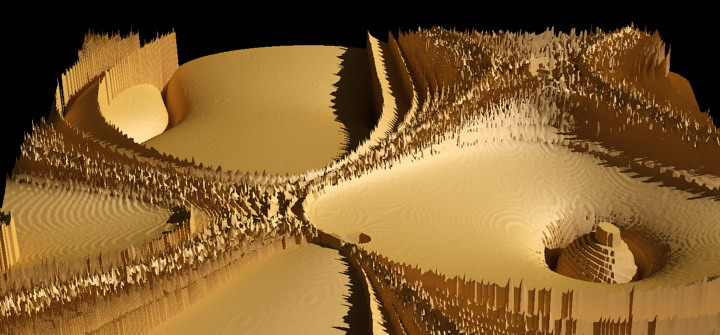
\includegraphics[width=0.32\linewidth]{imgs/tp04a_450}
 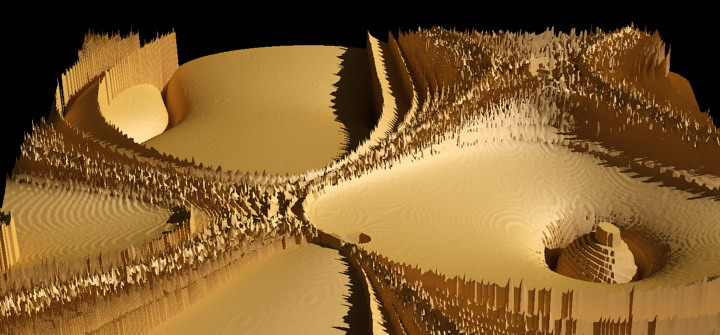
\includegraphics[width=0.32\linewidth]{imgs/tp04a_450}
 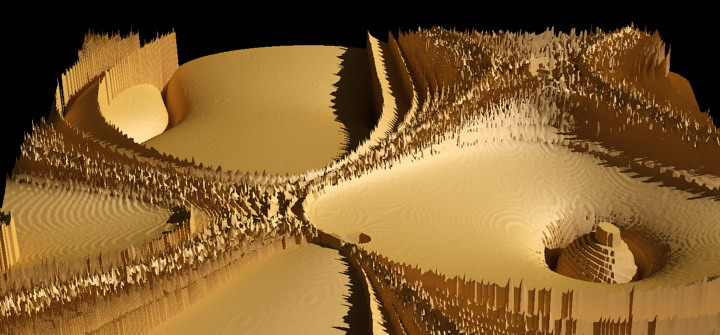
\includegraphics[width=0.32\linewidth]{imgs/tp04a_450}
 % tp04a_450.jpg: 720x335 pixel, 72dpi, 25.40x11.82 cm, bb=0 0 720 335
 \caption[curta]{Imagem composta por três figuras em ficheiros separados}
 \label{fig:terrenos}
\end{figure}


\begin{figure}
 \centering
 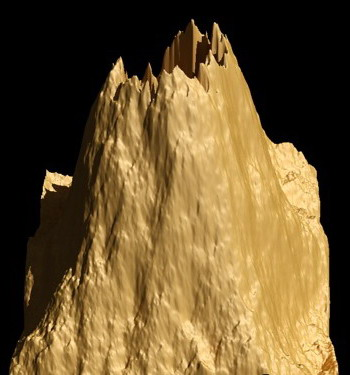
\includegraphics[width=0.5\linewidth]{imgs/tp45a_450}
 % tp45a_450.eps: 1179666x1179666 pixel, 300dpi, 9987.84x9987.84 cm, bb=20 20 575 615
 \caption{Vulcão}
 \label{fig:volcao}
\end{figure}


Na Tabela \ref{tableBenchmark} temos um exemplo de uma tabela onde existem linhas que ocupam mais do que uma linha da tabela.

% TODO - falta fazer isto!

\begin{table}
  \caption[exemplo de uma tabela]{Floating point benchmark.
	\textbf{R$_{max}$}: the performance in Gflops for the largest problem run on a machine;
	\textbf{N$_{max}$}: the size of the largest problem run on a machine;
	\textbf{N$_{1/2}$}: the size where half the R$_{max}$ execution rate is achieved;
	\textbf{R$_{peak}$}: the theoretical peak performance in Gflops for the machine}
  \label{tableBenchmark}
  \begin{center} 
  \begin{tabular*}{1\textwidth}{@{\extracolsep{\fill}} rccccc } \toprule
\textbf{Linpack	Benchmark}& Proc.	& \textbf{R$_{max}$} & \textbf{N$_{max}$} & \textbf{N$_{1/2}$}	& \textbf{R$_{peak}$} \\ 
(Full precision)	& or Cores	& GFlops	     & Order		  & Order		& GFlops \\ [0.25ex] \midrule
Thinking Machine CM-5	& 32		& 1,900		     & 9216		  & 4096		& 4 \\
Pentium 4 3.0 GHz & 1	& 4,730		     & 7600		  & 365			& 6 \\
\multirow{2}{*}{IBM Cell BE 3.2 GHz} 	& \multirow{2}{*}{9}& \multirow{2}{*}{98,05} & \multirow{2}{*}{4096} & \multirow{2}{*}{1536} & 204,8 {\scriptsize{(32 bits)}} \\
			&		&		     &			  &			& 14,6 {\scriptsize{(64 bits)}} \\ \bottomrule
  \end{tabular*}
  \end{center}	
\end{table}



As técnicas evolutivas baseiam-se em algoritmos bio-inspirados que aplicam a teoria de Darwin \parencite{Darwin1859}. Esta defende a evolução natural das espécies onde os organismos vivos são recompensados, através da sobrevivência e da propagação dos seus próprios genes aos sucessores. Actualmente existem quatro classes principais de algoritmos evolutivos: Algoritmos Genéticos (AG) \parencite{Holland1975}, Estratégias Evolutivas, Programação Genética (GP) \parencite{Koza1992} e Programação Evolutiva. Todos os algoritmos evolutivos mantêm uma população de soluções candidatas sobre a qual efectuam uma pesquisa para determinar os indivíduos mais fracos. De acordo com um determinado critério, estes são substituídos por outros gerados através de operadores aplicados aos melhores indivíduos da população, criando assim uma nova geração. Este processo é repetido sobre sucessivas gerações até se encontrar uma boa solução, que pode não ser a óptima.

Existem vários trabalhos e até video jogos que usam algoritmos evolutivos \parencite{Sims1992,url_Spore}.

\section{Incluir código fonte}
Nas Listagens \ref{ls:fibonacci} e \ref{ls:bash} temos um exemplo da inclusão de código fonte diretamente a partir do ficheiro fonte. Para mais informação ler o Manual da packge minted \parencite{Rudolph2016}. Nestes exemplos a formação foi configurada no ficheiro \texttt{config.tex} (procurar por \texttt{minted}). 


\begin{listing}[H] % quando cabe numa só página
    \caption{Código fonte C com sintaxe colorida}
    \label{ls:fibonacci}
    \codefilec{Code/fibonacci.c}
\end{listing}


\begin{longlisting} % quando ocupa mais que uma página
    \caption{Código fonte Bash que ocupa \underline{mais que uma página}}
    \label{ls:bash}
    \codefilebash{Code/bash.sh}
\end{longlisting}



Também é possível incluir código diretamente no ficheiro \LaTeXe, como no exemplo em baixo. A numeração das linhas é importante para ser possível referir o número da linha numa descrição.



\begin{listing}[H]
    \caption{Código fonte Python com sintaxe colorida}
    \label{ls:bash}
    \begin{pythoncode}
import numpy as np

def incmatrix(genl1,genl2):
    m = len(genl1)
    n = len(genl2)
    M = None #to become the incidence matrix
    VT = np.zeros((n*m,1), int)  #dummy variable

    #compute the bitwise xor matrix
    M1 = bitxormatrix(genl1)
    M2 = np.triu(bitxormatrix(genl2),1) 

    for i in range(m-1):
        for j in range(i+1, m):
            [r,c] = np.where(M2 == M1[i,j])
            for k in range(len(r)):
                VT[(i)*n + r[k]] = 1;
                VT[(i)*n + c[k]] = 1;
                VT[(j)*n + r[k]] = 1;
                VT[(j)*n + c[k]] = 1;

                if M is None:
                    M = np.copy(VT)
                else:
                    M = np.concatenate((M, VT), 1)

                VT = np.zeros((n*m,1), int)

return M
    \end{pythoncode}
\end{listing}
